%!TEX root = farm.tex

\section{Compiler and Debugging Environment}\label{sec:design}

This section describes the design and implementation of our compiler and
debugging environment for NVIDIA's GPU microcontrollers.

\subsection{Microcontroller}

\begin{table}[tb]
\caption{Specification of GF100 microcontroller.} 
\label{tab:fermi}
\hbox to\hsize{\hfil
\begin{tabular}{|l|r|r|}\hline
Name 		&	HUB	   & GPC\\\hline
Architecture &	Fermi   & Fermi \\\hline
Number of units	& 1 & 4\\\hline
Bit 		&	32bit  & 32bit\\\hline
Code size  &	16,384 byte  & 8,192 byte\\\hline
Data size  &	4,096 byte  & 2,048 byte\\\hline
% \multicolumn{4}{l}{type-1\,: enumerate$BEy(B\quad type-2\,: enumerate*$BEy(B}\\
% \multicolumn{4}{l}{type-3\,: Enumerate$BEy(B\quad type-4\,: ENUMERATE$BEy(B}\\
\end{tabular}\hfil}
\end{table}

This paper presumes the microcontroller of NVIDIA's Fermi architecture.
In particular, we target the GeForce GTX 480 graphics card designed
based on the GF100 architecture.
In this architecture, a streaming multiprocessor (SM) consists of
32 CUDA cores, while a graphics processing cluster (GPC) consists of 4
SM's.
There are four GPC's in total equipped in the GF100 architecture, and
hence the maximum number of CUDA cores is 512.

Table~\ref{tab:fermi} illustrates the specification of the GF100
microcontroller.
There are two types of microcontrollers, HUB and GPC, relevant to CUDA
engines.
HUB is broadcasting the access to all GPC's, while the GPC represents a
specific microcontroller for each GPC engine.
Since the maximum code size is limited to 16KB as indicated in Table
\ref{tab:fermi}, developers should carefully design the firmware.

\subsection{Compiler Implementation}

\begin{figure*}
\begin{center}
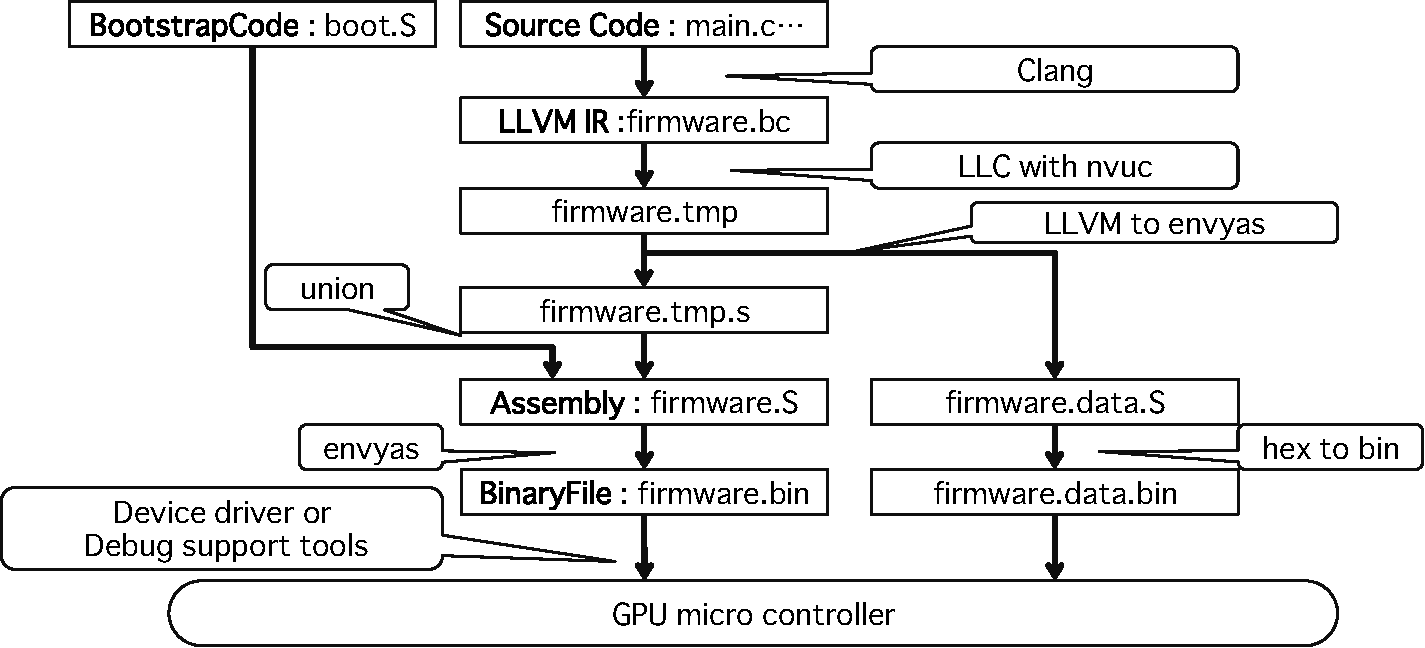
\includegraphics[width=12cm]{./img/step_compiler.pdf}
\end{center}
\caption{Overview of Compiler Implementation.}
\label{fig:compiler}
\end{figure*}

Figure \ref{fig:compiler} shows an overview of our compiler
implementation.
The main flow of compilation is done by Clang.
It generates the LLVM IR from the C source file.
The LLC next generates assembly code, which contains code and data in
separate files.
Finally, the Envytools outputs an executable file.
This executable file can be launched by the device driver, and can also
be tested by our debugging tool described in the later section.
To summarize, our compiler takes the following stages:

\begin{figure}
 \begin{center}
  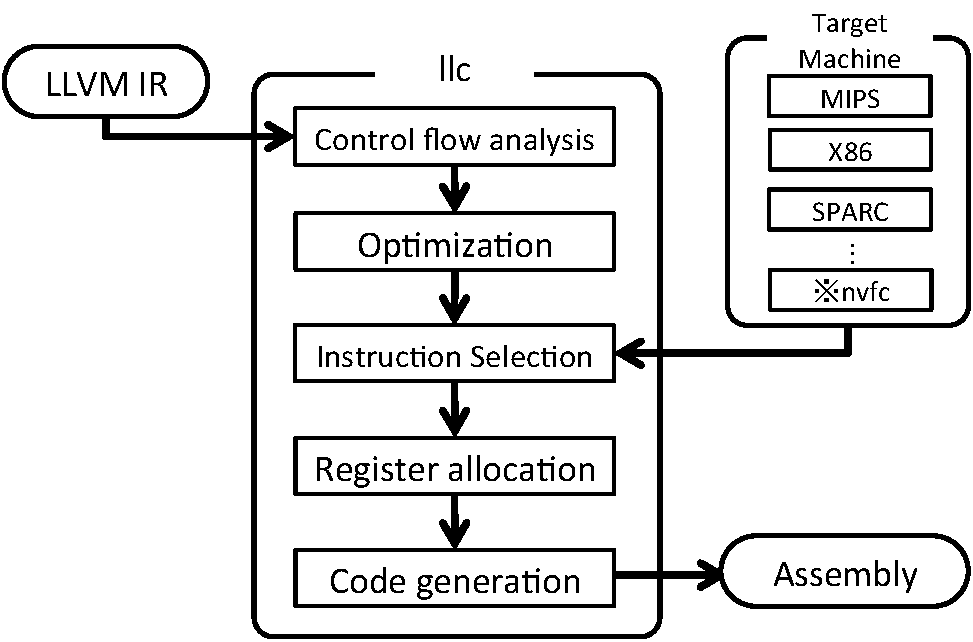
\includegraphics[width=6cm]{./img/llc.pdf}
 \end{center}
 \caption{Code generation stages of LLC.}
 \label{fig:llc}
\end{figure}

\begin{figure*}
 \begin{center}
  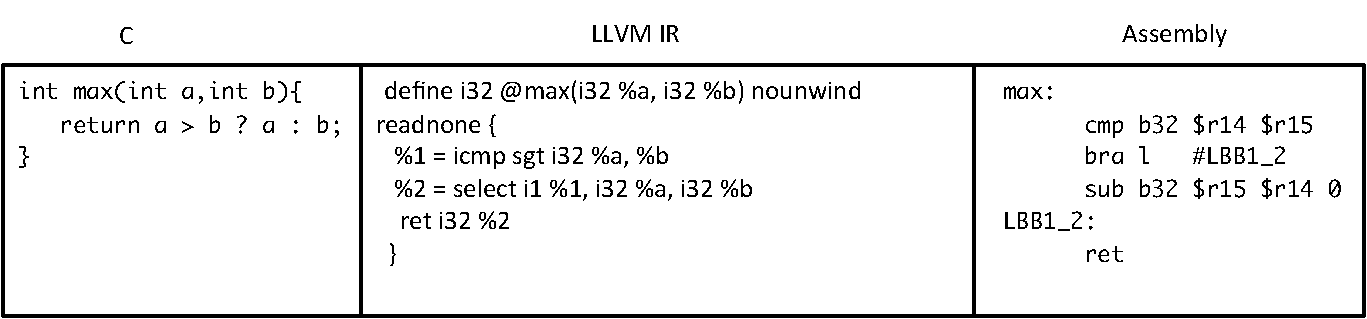
\includegraphics[width=12cm]{./img/llvm_code.pdf}
 \end{center}
 \caption{Examples of C source code and output code.}
 \label{fig:llvm_code}
\end{figure*}

\begin{description}
\item[ (1) Clang]\mbox{}\\
	   This is a frontend of C language that generates LLVM IR code
	   from the source file.

\item[ (2) LLC with nvuc]\mbox{}\\
	   This is a backend of LLVM that compiles LLVM IR code into
	   assembly code. 
	   As shown in Figure~\ref{fig:llc}, there are five steps to
	   exploit compilation: (i) flow analysis, (ii) optimization,
	   (iii) instruction selection, (iv) register allocation, and
	   (v) code generation.
	   This flow is not dependent on the target machine.
	   The LLC reads a configuration of the target machine at the
	   time of instruction selection, and selects a set of the
	   instruction and register to meet the specifications of each
	   machine.
	   Our implementation adds a new configuration called nvuc
	   (NVIDIA Micro-Controller) to support NVIDIA's GPU
	   microcontrollers under the LLVM infrastructure.

\item[ (3) LLVM to envyas]\mbox{}\\
	   This stage divides the generated assembly code into code and
	   data sections so that we can create binary images using
	   ``envyas'', which is a microcontroller assembler provided by
	   the Envytools suite.
	   The bootstrap code is also unified into the binary images
	   in this stage.
\item[ (4) envyas]\mbox{}\\
	   This is a final assembly stage for the microcontroller, which
	   generates the byte code of the firmware.
\item[ (5) hex to bin]\mbox{}\\
``hex to bin'' converts to the data portion split Step (3) to an executable file.

\item[ (6) Running the firmware]\mbox{}\\
There are two ways to run the firmware: incorporating the firmware into the device driver, or using the debugging support tool.
The device driver and the debugging support tool load the binary file of the firmware at boot time.
\end{description}

Figure \ref{fig:llvm_code} shows example of C language source codes, LLVM IR code, and assembly code.
Left is C language source codes, center is LLVM IR code that is generated by \ref{section:flow}(1), right is assembly code that is generated by \ref{section:flow}(3).

\begin{figure}
\begin{center}
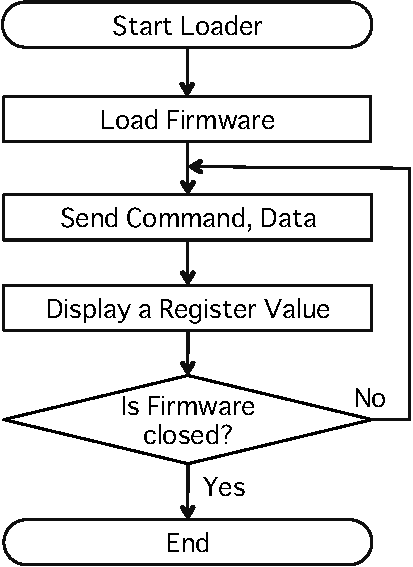
\includegraphics[width=3cm]{./img/loader.pdf}
\end{center}
\caption{Flowchart of Debugging Support Tool}
\label{fig:loader}
\end{figure}

\begin{figure*}
\begin{center}
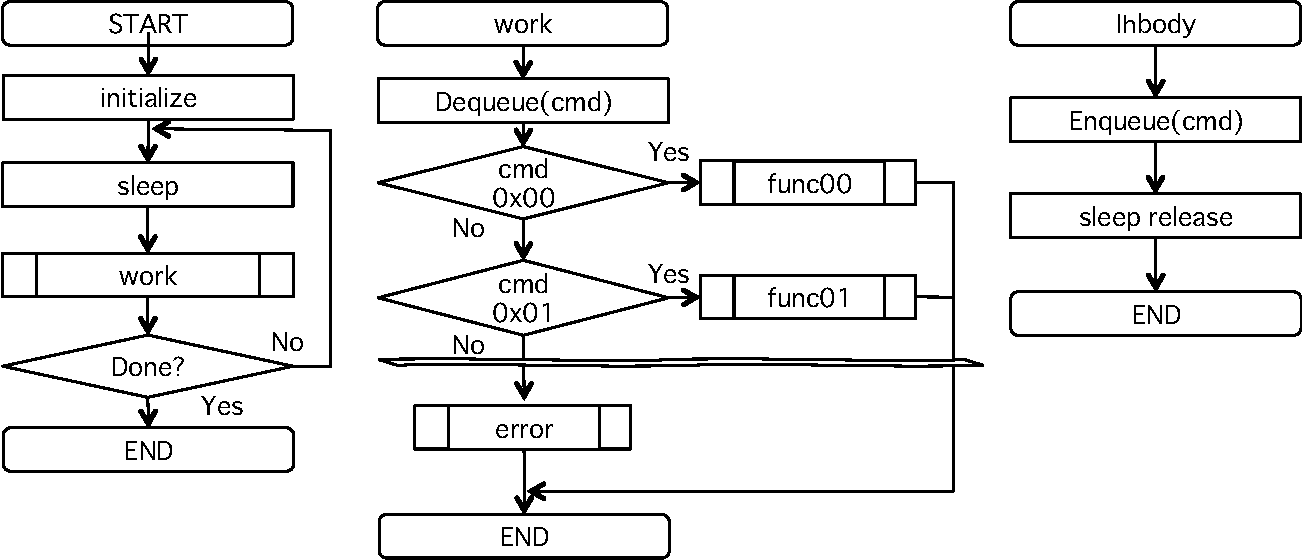
\includegraphics[width=12cm]{./img/firmware.pdf}
\end{center}
\caption{Flowchart of Our Firmware }
\label{fig:firmware}
\end{figure*}


\subsection{Debugging support tool}
Debugging support tool is to load the firmware, to send commands and data, and to display a register value of GPU.
Figure \ref{fig:loader} shows the flow of this tool flow, we describe use it.
Microcontrollers memory space map to  CPU memory space in MMIO (Memory Mapped IO).

\begin{description}
\item[ (1) Load the firmware]\mbox{}\\
Debugging support tool load the HUB firmware and GPC firmware executable code to mapping address by MMIO. 
After the load completion, this firmware runs by set a flag in the specified register.
\item[ (2) Sends commands and data]\mbox{}\\
A processing on microcontroller is suspended until receives a command.
The debugging support tool sends the command.
After an interrupt is executed by the command, the processing is resumed,

\item[ (3) Display a register] \mbox{}\\
The microcontroller has the register may be used freely on the host side.
The register is used for execute completion flag by the traditional firmware.
Thus we assumed that the register is used for the same purpose during debugging time, 
the register value is displayed.
\end{description}


\subsection{Firmware development}
In this section, we describe the our developing firmware on HUB.
Figure \ref{fig:firmware} shows that firmware flow chart.
The Firmware is started by setting the value in the register.

\begin{description}
\item[ (1) initialize]\mbox{}\\
The firmware sets the interrupt handler and get the data when started.
Next then Step(2).
\item[ (2) sleep]\mbox{}\\
The firmware makes the shift to the standby state, which wait for the receive command by the device driver or the debug support tools.
The firmware interrupt occurs when the firmware received command, which started ``ihbody''. 

\item[ (3) ihbody] \mbox{}\\
``ihbody'' enqueued command, and then it releases wait state of firmware.
\item[ (4) work] \mbox{}\\
``work'' function is called when the wait state of firmware is released.
``work'' calls the function after the dequeue.
It will check the end flag of firmware after the function execution.
\end{description}
We can recognize from what has been said that the firmware controlled by execute the function is better suited command.

